\documentclass{beamer}
%
% Choose how your presentation looks.
%
% For more themes, color themes and font themes, see:
% http://deic.uab.es/~iblanes/beamer_gallery/index_by_theme.html
%
\mode<presentation>
{
  \usetheme{default}      % or try Darmstadt, Madrid, Warsaw, ...
  \usecolortheme{default} % or try albatross, beaver, crane, ...
  \usefonttheme{default}  % or try serif, structurebold, ...
  \setbeamertemplate{navigation symbols}{}
  \setbeamertemplate{caption}[numbered]
} 


\usepackage[english]{babel}
\usepackage[utf8x]{inputenc}


\title[Your Short Title]{Neizrazita logika u vremenskim nizovima}
\author[Vinko Kolobara]{Vinko Kolobara\\{\footnotesize Mentor: prof.dr.sc Domagoj Jakobović}}
\institute{Fakultet Elektrotehnike i Računarstva, Zagreb}
\date{24.01.2018}

\setbeamertemplate{footline}[frame number] 

\AtBeginSection[]{
  \begin{frame}[plain,noframenumbering]
  \vfill
  \centering
  \begin{beamercolorbox}[sep=8pt,center,shadow=true,rounded=true]{title}
    \usebeamerfont{title}\insertsectionhead\par%
  \end{beamercolorbox}
  \vfill
  \end{frame}
}

\begin{document}

\begin{frame}[plain,noframenumbering]
  \titlepage
\end{frame}

% Uncomment these lines for an automatically generated outline.
\begin{frame}[plain,noframenumbering]{Outline}
  \tableofcontents
\end{frame}


\section{Neizrazita logika}

\subsection{Uvod}
\begin{frame}{Uvod}

\begin{itemize}
  \item uvodi nesigurnost, neizrazitost u klasičnu logiku
  \item omogućuje definiranje pravila u "ljudskom" jeziku
  \item neizraziti skupovi
  \item svaki element skupa pripada skupu s nekim stupnjem pripadnosti (funkcija pripadnosti )
\end{itemize}

\end{frame}

\begin{frame}{}
\begin{figure}[h]
  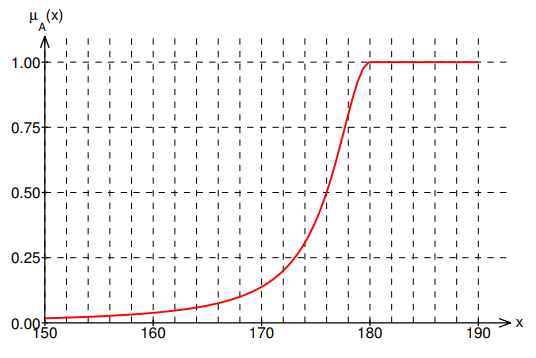
\includegraphics[width=\textwidth]{img/fuzzy_tall.png}
  \caption{Neizraziti skup koji predstavlja izraz "visok čovjek"}
\end{figure}
\end{frame}

\subsection{Jezične varijable}

\begin{frame}{Jezične varijable}
\begin{itemize}
  \item uređena n-torka $(X, T_X, U, G, M_X)$
  \item definira određeni pojam, npr. "visina"
  \item sastoji se od jezičnih izraza, npr: "patuljast", "nizak", "umjeren", "visok", "jako visok", "Yao Ming"
  \item jezični modifikatori: "vrlo", "otprilike"
\end{itemize}
\end{frame}

\begin{frame}{}
\begin{figure}[h]
  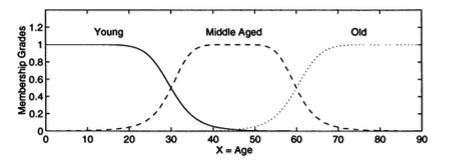
\includegraphics[width=\textwidth]{img/fuzzy_var.png}
  \caption{Neizrazita varijabla "starost"}
\end{figure}
\end{frame}

\subsection{Neizrazito zaključivanje}
\begin{frame}{Neizrazito zaključivanje}

\begin{itemize}
  \item ako-onda pravila
  \item \textbf{implikacija, s-norma, t-norma, komplement}
  \item više vrsta zaključivanja: Mamdani, TSK
\end{itemize}
\end{frame}

\begin{frame}{}
\begin{figure}[h]
  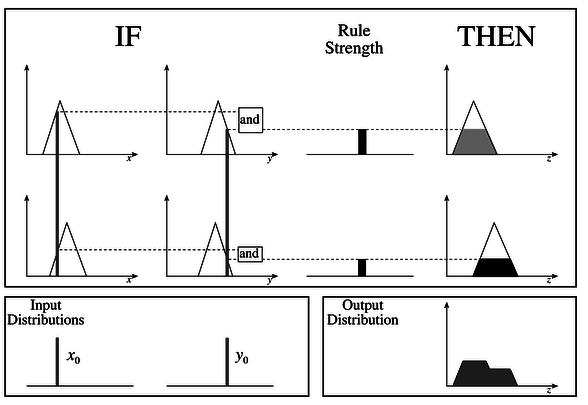
\includegraphics[width=\textwidth]{img/fuzzy_inf.png}
  \caption{Primjer Mamdani zaključivanja}
\end{figure}
\end{frame}

\begin{frame}{DEMO}
% TODO: UBACI SVOJA PRAVILA I DEFINICIJE
\end{frame}



\section{ANFIS}

\begin{frame}{}
\begin{figure}[h]
  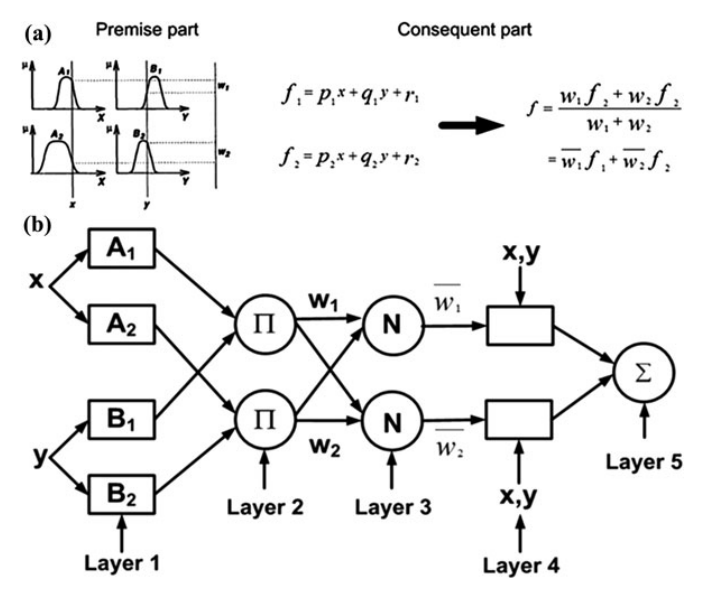
\includegraphics[width=\textwidth]{img/anfis.png}
\end{figure}
\end{frame}

\begin{frame}{}

\begin{itemize}
  \item neuronske mreže + neizrazito zaključivanje
  \item uči pravila
  \item backpropagation, evolucijski algoritmi
\end{itemize}
\end{frame}

\section{Čemu to?}

\begin{frame}{}
\begin{figure}[h]
  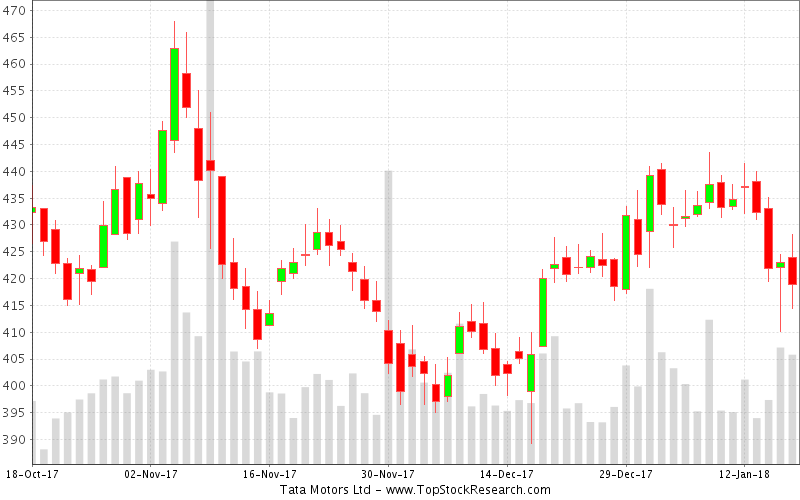
\includegraphics[width=\textwidth]{img/candlestick.png}
\end{figure}
\end{frame}

\begin{frame}{Tehnički indikatori}

\begin{itemize}
  \item trend - moving averages, MACD
  \item momentum - CCI, RSI
  \item volatilnost - Bollinger Bands
  \item opseg trgovine (volume) - OBV, ROCV
  \item sentiment - u jako volatilnim tržištima (kriptovalute)
\end{itemize}
\end{frame}

\begin{frame}{Ideja}
\begin{itemize}
  \item pomoću tehničkih indikatora razviti strategiju trgovanja AKO-ONDA pravilima
  \item pomoću uzoraka koji se pojavljuju razviti strategiju ili pronaći nove uzorke
\end{itemize}
\end{frame}

\begin{frame}{}
\begin{figure}[h]
  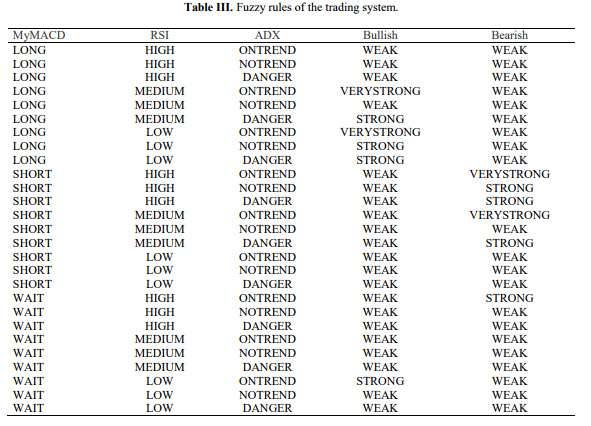
\includegraphics[width=\textwidth]{img/fuzzy_rules.png}
\end{figure}
\end{frame}

\begin{frame}{Abandoned baby 1}
\begin{figure}[h]
  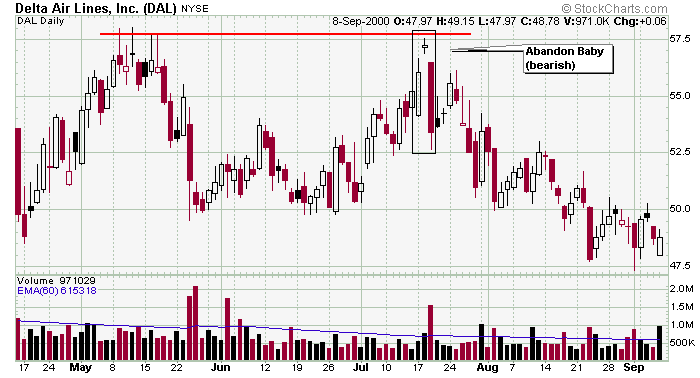
\includegraphics[width=\textwidth]{img/baby1.png}
\end{figure}
\end{frame}

\begin{frame}{Abandoned baby 2}
\begin{figure}[h]
  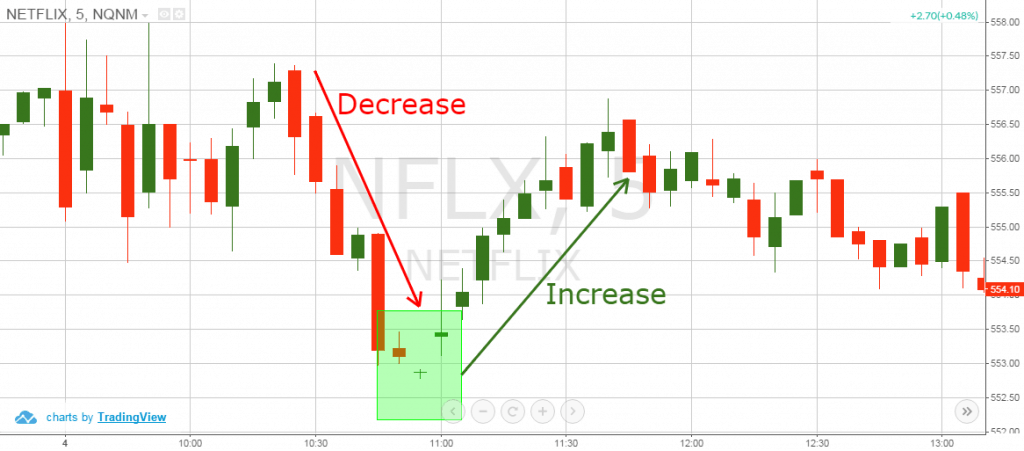
\includegraphics[width=\textwidth]{img/baby2.png}
\end{figure}
\end{frame}

\begin{frame}{Abandoned baby 3}
\begin{figure}[h]
  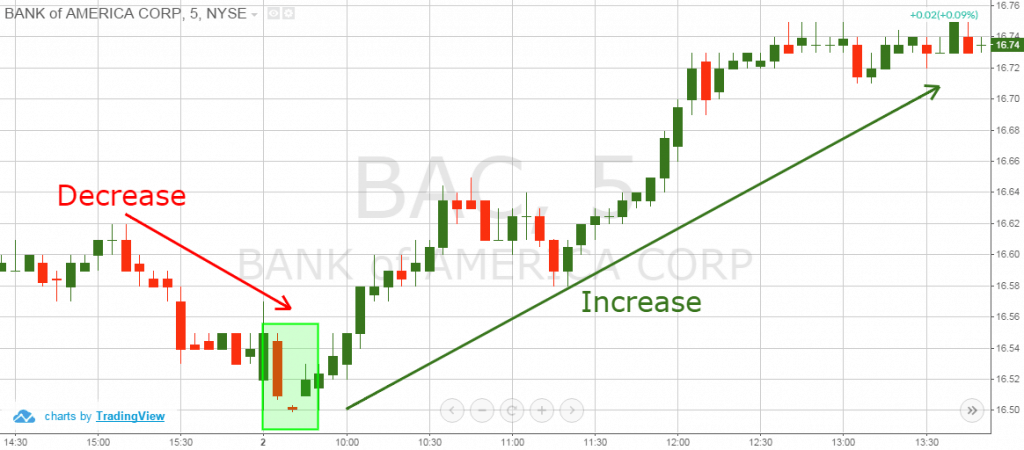
\includegraphics[width=\textwidth]{img/baby3.png}
\end{figure}
\end{frame}

\begin{frame}[plain, noframenumbering, allowframebreaks]
  \frametitle<presentation>{Further Reading}    
  \begin{thebibliography}{10}    
  \bibitem{cupic}
    Čupić, Marko; Bašić Dalbelo, Bojana i Golub, Marin
    \newblock {\em Neizrazito, evolucijsko i neuroračunarstvo}.
  \bibitem{trading_system}
    Naranjo, Rodrigo; Meco, Albert; Arroyo, Javier i Santos, Matilde
    \newblock {\em An Intelligent Trading System with Fuzzy Rules and Fuzzy Capital Management}.
  \bibitem{fin}
    Ruey S. Tsay
    \newblock {\em Analysis of Financial Time Series}    
  \end{thebibliography}
\end{frame}

\end{document}
